\chapter{Prototyping the device}
\label{Chap:Prototype}
Once we have the parts we selected,
we need to connect them correctly so that they can communicate with each other.
Most electronic components are accompanied by a datasheet created by its manufacturer.
This datasheet details the behaviour of the component,
its electrical and non-electrical characteristics,
its physical design,
pin layout,
and a typical application circuit.
This typical application circuit allows us to connect the component in the way intended by its manufacturer.
An example of this application circuit is a clipping shown in figure \ref{Fig:MPUAppCircuit} from the datasheet \cite{Datasheet:MPU6000} for the MPU-6000.
\begin{figure}
\begin{center}
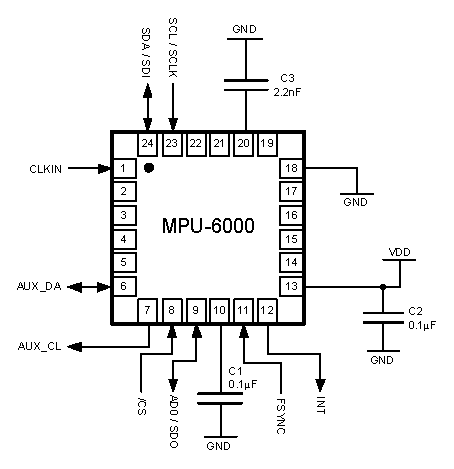
\includegraphics{images/MPU600OpCircuit.eps}
\caption{Typical Operating Circuit for the MPU-6000}
\label{Fig:MPUAppCircuit}
\end{center}
\end{figure}
As we can see,
the typical application circuit for the sensor shows us the pin layout of the chip,
along with any external components that need to be connected.
In this case, it shows three capacitors that must be connected to the chip.
Similar to the MPU-6000,
all the components we have selected for our device design have their respective datasheets which contain information on how they should be operated.
Using these datasheets,
a master circuit was created for our device.
This circuit was designed in the EAGLE PCB Design software.

\section{Overview}
\label{Sec:PCBDesign}
All components in the final device will be connected to each other using a Printed Circuit Board.
PCB's replace wires between components by copper traces on the board,
which are lines made of wire that can conduct electricity.
Creating a PCB requires three steps, the first being circuit design.
Once the circuit is designed, the components are laid out on a PCB, and traces are created based on the circuit design.
The third process comprises of of using this layout to create the actual PCB.
This third step is completed by PCB manufacturers after we provide them with our PCB layout design.
The benefit of creating a schematic in EAGLE instead of directly creating a layout connected by traces
is that the software uses the connections in the schematic to guide us while connecting the pins or pads of the different components.
This reduces the chances of an incorrect connection between two components,
reducing any mistakes that might creep into our final PCB design and cost us money as we re-manufacture our PCB.
\begin{figure}
\begin{center}
\includegraphics[width=0.8\textwidth]{images/EagleScreen.jpg}
\caption{Screenshot of EAGLE PCB's schematic editor.}
\label{Fig:EaglePCBScreen}
\end{center}
\end{figure}

\section{Unit Testing}
\label{Sec:UnitTesting}
Before we connect all our devices together,
we need to test each component seperately and make sure they work as expected.
Although most parts have a low failure rate,
it is easier to work through with our devices knowing where a bug is,
if one shows up during the creation process.
Unit Testing is a method of testing individual units of source code to check if they work as expected before introducing them into a larger piece of code.
We extend this to our device creation process by testing each unit of hardware seperately.
We would have to test the microcontroller, the sensor, the memory chip, the USB to UART bridge and the battery charger.
The microcontroller would have to be the first component to be tested because the other components require a master device that controls them.

\subsection{Micrcontroller Testing}
To test the microcontroller we used a simple "Hello World" program.
Since microcontrollers do not have a display, instead of displaying text,
it is easier to just blink an LED using one of the pins.
Pseudocode to blink the LED is showin in listing \ref{LST:LEDHello}.
We programmed our microcontroller using IAR's Code Composer Studio,
and then flashed the microcontroller using the software and the MSP430 Flash Emulation Tool.
If our connections were correct,
the LED would turn on for one second,
then turn off for another second.
This cycle would repeat indefinitely, creating the illusion of a light blinking slowly.
\begin{lstlisting}[caption=My caption,label=LST:LEDHello]
/* We want to blink forever */
while(1)
{
	/* Create a delay. Our clock is at 32768 Hz */
	__delay_cycles(32768);
	FlipLEDStatus();  
}
\end{lstlisting}
\subsection{Sensor Testing}
\label{Sec:SensorTesting}
\begin{figure}
\begin{center}
\includegraphics[width=0.6\textwidth]{images/Cat5Twist.jpg}
\caption{REPALCE WITH MPU6000 CAT5}
\label{Fig:CAt5MPU}
\end{center}
\end{figure}

After confirming that the microcontorller chip is performing as expected,
we need to check our sensor. We talked about Breakout Boards \ref{Sec:Breakouts} earlier,
which allow us to prototype sensors without worrying about soldering them.
Breakout boards for the MPU-6000 were obtained from an Ebay seller.
The breakout board has 6 pins that need to be connected for operation,
which means we need 6 wires between the microcontroller and the breakout board.
These pins on the breakout board were connected to the microcontroller target board using a CAT5 cable as can be seen in figrure \ref{FIG:Cat5MPU}.
This is the same cable used for Ethernet connections, and thus was easy to obtain.
As shown in the same figure,
a regular CAT5 cable consists of 4 pairs of twisted wires,
so one pair in this cable would not be used.
This pair was connected to the GND pin on the microcontroller to reduce noise.

Our sensor uses SPI for communication.
The datasheet mentions that once the sensor is powered on and woken from sleep mode,
the sensor will start recording what the acceleration and angular velocity are.
This information is storing in an internal memory on the sensor which can be read using SPI instructions.
We initially had trouble verifying if our sensor is working correctly and did not know if the sensor was faulty,
or if there was a mistake in our connections or code.
The datasheet for the sensor mentions a register called ``WHO\_AM\_I'' which containst he device's I$^2$C address.
This address by default is set to 0x68.
Since this register contains a constant number, we can read it to check if the device is indeed correctly connected.

After some troubleshooting we learnt that the length of the cable was too long for SPI communication and signals would strength.
Also, SPI is time sensitive, so if the cable length was too long,
the delay created between two times would be too high,
causing incorrect data to be received.
We fixed this by reducing how long the cable was.
In the final design the length the signal would have to travel would be very small since the chips would be laid out next to each other,
so this was not an issue we needed to worry about.
Once it was established that the sensors were working correctly and SPI communication between them was also as expected,
we carried out simple tests where the acceleration on one axis would turn an LED on if positive,
otherwise turn it off.
Since gravity would show as -1g on the Z Axis in the Earth Frame of reference,
we could test all three sensor axes by rotatin the sensor and observing the LED's behaviour.
These tests concluded that communication between the sensor and microcontroller was as expected.

\subsection{Memory Chip Testing}
\label{Sec:MemoryTesting}
Similar to the sensor, we needed to test our memory chip and make sure SPI communication was up and running.
As seen in Section \ref{Sec:Memory},
we created our own breakout board to break the pins out from the memory chip.
To check if SPI communication was running fine,
we used a method similar to what was used for the sensor.





















\section{Circuit Design}
\label{Sec:CircuitDesign}
Now that we know what the different typical operating cicruits for each device look like,
and that they work as expected with the microcontroller,
we need to connect all of these devices to each other.
The circuits for different parts of the device that we designed are shown in figures X, Y, Z and E.
The circuit we designed after consulting the different datasheets is shown in figure \ref{Fig:CompleteCircuit} in the Appendix.
This circuit was created using EAGLE PCB's schematic layout tool.
Each component had its circuit created seperately,
and later these circuits were connected together to create the final device.
A screenshot of Eagle PCB's schematic editor is shown in figure \ref{Fig:EaglePCBScreen}.
\begin{figure}
\begin{center}
\includegraphics[width=0.8\textwidth]{images/EagleScreen.jpg}
\caption{REPLACE WITH PHOTO OF BREADBOARD PROTOTYPE}
\label{Fig:BreadBoardProto}
\end{center}
\end{figure}

Once this circuit was ready, we used a breadboard to prototype the device.
A breadboard is a board with holes in a dot matrix arrangement.
Through hole components can be mounted on this board.
Some holes on the breadboard are connected to each other,
which allows the connection of components without the use of wires when placed correctly.
The breadboard allowed us to connect our components together and program the microcontroller with a reduced amount of soldering, 
and this can be seen in figure \ref{Fig:BreadBoardProto}.

\section{Programming}
\label{Sec:Programming}
Now that we had all our components connected together on the breadboard,
it was possible to program our microcontroller and make it perform its required functions.
As described in Hardware Selection (section \ref{Sec:Hardware}),
our program would poll the sensors repeatedly.
The data from these sensors would be stored in the microcontrollers memory till the total data crossed a threshold.
Once this threshold was crossed, the data would be sent to the memory chip.
A simplified version of the microcontrollers code is seen in figure \ref{Fig:MainAlgo}.


\subsection{PCB Layout}


\label{Sec:Software}

\subsection{Soldering}
\label{Sec:Soldering}
